\chapter{Introduction}

With each year new companies jumping into the \emph{IoT} sector and all the
major \emph{IT actors} investing in the development of new
products\footnote{\url{https://www.fortunebusinessinsights.com/industry-reports/internet-of-things-iot-market-100307}},
as well as telecoms building infrastructure for this new 
demand\footnote{\url{https://www.proximus.be/en/id_cl_iot/companies-and-public-sector/it-services/iot/internet-of-things.html}}
The \emph{Internet of Things}, describing interconnected devices gathering
data without human interaction, has undoubtedly been a subject of hype during the
last decade while maintaining a consistent growth until now.
Business analysts agree that we should expect to reach at least 40 billion
installed \emph{IoT} devices by
2027\footnote{\url{https://www.businessinsider.com/internet-of-things-report}}. 
Consumers are already familiar with the traditional \emph{IoT} products
we use in our households. They allow to connect our light bulbs, our fridge and
washing machine, \ldots
Meanwhile we have less knowledge of the industrial usage of \emph{IoT}, also
known as \emph{IIoT}. \emph{IIoT} is one of the fastest growing domain of the
market. More and more industries are adopting \emph{IoT}  to consolidate their
productions with \emph{real-time monitoring}, predictive maintenance on their
assets and products, connecting their supply chains, all of this enabled with
the help of network of sensors, in a wide variety of
sectors like \emph{smart farming}, \emph{smart cars}, \emph{smart cities},
\emph{energy managements}, \ldots

\paragraph{}

The common aspect of all of these applications are that they can communicate
wirelessly.
A multitude of telecommunication technologies are used or were created to suit
this solution and can be categorized by three different characteristics.

\begin{itemize}
    \item Long or Short \emph{range}
    \item High or low \emph{data-rate}
    \item Low or high \emph{power usage} 
\end{itemize}

% From these characteristics you can only chose two according to the physical
% law. % TODO Explanation needed with the exact law reference explaining this
The following graphics (Fig~\ref{fig:commrangegraph}) show a classification of
existing wireless communication protocol used in the \emph{IoT} and mix it in three 
main categories.

\begin{itemize}
    \item \emph{Short-Range wireless communication} Short range, high data-rate
    \item \emph{Cellular communication} Long range, high data-rate
    \item \emph{LPWAN communication} Long range, low power and low data-rate
\end{itemize}

\begin{figure}[H] % TODO More info on axis
\centering
\begin{tikzpicture}
    \draw[->,thick] (-0.1,0)--(12,0) node[right]{Range};
    \draw[->,thick] (0,-0.1)--(0,8) node[above]{Data Rate};
    \node[] at (1, -0.5) {10m};
    \draw[] (1,-0.1)--(1,0.1);
    \node[] at (3, -0.5) {100m};
    \draw[] (3,-0.1)--(3,0.1);
    \node[] at (5, -0.5) {1km};
    \draw[] (5,-0.1)--(5,0.1);
    \node[] at (7, -0.5) {10km};
    \draw[] (7,-0.1)--(7,0.1);
    \node[] at (9, -0.5) {100km};
    \draw[] (9,-0.1)--(9,0.1);

    \node[] at (-1.2, 1) {1 kbit/sec};
    \draw[] (-0.1,1)--(0.1,1);
    \node[] at (-1.2, 3) {1 Mbit/sec};
    \draw[] (-0.1,3)--(0.1,3);
    \node[] at (-1.2, 5) {100 Mbit/sec};
    \draw[] (-0.1,5)--(0.1,5);
    \node[] at (-1.2, 7) {1 Gbit/sec};
    \draw[] (-0.1,7)--(0.1,7);
    
    \node[draw] at (8,1.5) (lora) {LoRa};
    \node[draw] at (9.0,0.8) (sigfox) {SigFox};
    \node[draw] at (7.4,2.2) (nb) {NB-IOT};
    \node[draw,dotted,fit=(lora) (sigfox) (nb), label=above:{LPWAN}] {};

    
    \node[draw] at (2.2,3.5) (bluetooth) {Bluetooth};
    \node[draw] at (2.7,2.5) (zigbee) {ZigBee};
    \node[draw] at (2.0,1.8) (ble) {BLE};
    \node[draw] at (3,5) (wifi) {WiFi};
    \node[draw,dotted,fit=(bluetooth) (zigbee) (ble) (wifi), label=above:{Short-range}] {};

    \node[draw] at (6.8,5) (lte) {LTE};
    \node[draw] at (5.8,6) (5g) {5G};
    \node[draw,dotted,fit=(lte) (5g), label=above:{Cellular}] {};
\end{tikzpicture}
\caption{Comparison of the existing IoT wireless technologies by range and data rate}
\label{fig:commrangegraph}
\end{figure}


This work focus only on \emph{LoRa}, a proprietary \emph{chirp spread spectrum}
modulation technique owned by \emph{Semtech}, operating in the sub-GHz
unlicensed \emph{ISM} band, that will be explained in more details in 
Section~\ref{section:lora}.
The main characteristics of \emph{LoRa} is that it trade throughput for range
and low power transmission. 
The long-range capabilities of the protocol has caught the attention of
many people with record distance transmission over 700 km
with direct line of sight between the receiver and the
transmitter\footnote{https://www.thethingsnetwork.org/article/ground-breaking-world-record-lorawan-packet-received-at-702-km-436-miles-distance}.
However, this case is not a real world example, we should still expect a typical 
range in urban areas of around \emph{2 to 5 km} and \emph{15 km} in suburban
areas~\cite{8030482}. Fine-tuning the \emph{PHY} settings of the protocol also
allow trading communication distance over throughput and a longer band usage,
which decrease the number of concurrent motes that can communicate over the
band~\cite{10.1145/2988287.2989163}.

\emph{LoRa} is often used in conjunction with the \emph{LoRaWAN} a 
point-to-multipoint protocols.
\emph{LoRaWAN} is a ALOHA based~\cite{loraalliance:lorawanspecification} network
using a star-of-stars topology composed of wirelessly interconnected 
\emph{motes} sending data to \emph{gateways}, relaying messages to central 
servers over a Cellular or Ethernet connection as we can see in 
Figure~\ref{fig:startopology}.
This single-hop topology is an easy to deploy solution because network coverage
for LoRaWAN is fairly
developed\footnote{\url{https://www.thethingsnetwork.org/map}}.

\begin{figure}[H]
\begin{subfigure}[b]{.5\textwidth}
    \centering
    \begin{tikzpicture}[auto, thick]
      % Place super peers and connect them
      \foreach \place/\name in {{(0,-1)/a}, {(2,0)/b}, {(2.5, -3)/c}}
        \node[gateways] (\name) at \place {};
      \node[server] (d) at (1.5,-1.5) {};
      %
      \foreach \source/\dest in {a/d, b/d}
        \path[dotted] (\source) edge (\dest);
      \path (c) edge (d); % Non dotted
      %
      % Place normal peers
      \foreach \pos/\i in {above right of/1, right of/2, below right of/3}
        \node[motes, \pos =b ] (b\i) {};
      \foreach \speer/\peer in {b/b1,b/b2,b/b3}
        \path[dotted] (\speer) edge (\peer);
      %
      \foreach \pos/\i in {below left of/1, below of/2, left of/3, above right of/4}
        \node[motes, \pos =a ] (a\i) {};
      \foreach \speer/\peer in {a/a1,a/a2,a/a3,a/a4}
        \path[dotted] (\speer) edge (\peer);
      %
      \path[dotted] (b) edge (a4);
    \end{tikzpicture}
    \caption{Star topology}
    \label{fig:startopology}
\end{subfigure}
\hfill
\begin{subfigure}[b]{.5\textwidth}
    \centering
    \begin{tikzpicture}[auto, thick]
      % Place super peers and connect them
      \foreach \place/\name in {{(0,-1)/a}, {(2,0)/b}, {(2, -3)/c}, {(1,1)/d}, {(1.5, -1.5)/f}}
        \node[motes] (\name) at \place {};
      \foreach \source/\dest in {a/b, a/c, b/c, d/b, f/a, f/b, f/c}
        \path[dotted] (\source) edge (\dest);
      %
      % Place normal peers
      \foreach \pos/\i in {above right of/1, right of/2, below right of/3}
        \node[motes, \pos =b ] (b\i) {};
      \foreach \speer/\peer in {b/b1,b/b2,b/b3}
        \path[dotted] (\speer) edge (\peer);
      %
      \foreach \pos/\i in {above left of/1, left of/2, above of/3}
        \node[motes, \pos =d ] (d\i) {};
      \foreach \speer/\peer in {d/d1,d/d2,d/d3}
        \path[dotted] (\speer) edge (\peer);
      %
      \foreach \pos/\i in {below left of/1, below of/2, left of/3}
        \node[motes, \pos =a ] (a\i) {};
      \foreach \speer/\peer in {a/a1,a/a2,a/a3}
        \path[dotted] (\speer) edge (\peer);
    \end{tikzpicture}
    \caption{Mesh Network Topology}
    \label{fig:meshtopology}
\end{subfigure}
\caption{Different LoRa Network Topologies}
\label{fig:topologies}
\end{figure}




The issue is that \emph{LoRaWAN} does not scale as studied 
in~\cite{8030482}~\cite{10.1145/2988287.2989163}. This occurs especially 
with dense networks, like in urban environments, where a lot of collision can
happen during transmission.

LoRaWAN is a \emph{ALOHA} based MAC protocol and channel sensing is impossible 
because \emph{Channel Activity Detection} (CAD) only detect the preamble of a 
communication. % TODO reference needed
This lead to collision when transmitting at the same time and until the message 
is correctly sent, the transmission has to be re-done.
We should then expect bigger energy consumption for the motes and bigger radio 
channel occupation.
As the network get more dense~\cite{8030482}, the effect of collision get 
increasingly significant with little to no packet getting received by a base
station.

The \emph{duty-cycle} regulations in place with the \emph{ISM} bands on every
transmitting devices (motes and gateways) is then a limiting factor 
for \emph{LoRaWAN} (\cite{8030482}).
The european ISM band has set a duty-cycle of \emph{1\%} meaning each node 
and gateway has a maximum transmission time per hour of \emph{36 sec/hour}. 
Increasing the number of retransmission of a packet quickly become impossible.
% TODO {Add some reference to ISM regulations} 

Link quality is also influencing on LoRaWAN efficiency. 
Motes on the limit of the gateway coverage may struggle to achieve a
complete transmission. 
Environmental factor like temperature, humidity as studied 
in~\cite{evaluation_of_the_reliability_of_lora}, the topology of the 
terrain~\cite{lorajambalaya}, influence a lot the link quality.
All these factor make the network coverage of a typical gateway not uniform 
as we can see in Fig~\ref{fig:coverage}.

Gateways can restrain the deployment of a LoRa network.
They may not be available to deploy everywhere and some use cases may not even allow
the installation of gateways because they require more demanding infrastructure 
than a battery operated mote.
That's the case for pipelines and tunnel as in~\cite{Abrardo_2019},
where we would prefer to only install motes running on batteries because a
gateway wouldn't have much effect with the linear nature of the installation.
They can also be a single point of failure of the network, when a single
gateway is connecting a portion of the network, in the event of a technical
issue this whole network will remain unconnected.

\begin{figure}[H]
    \centering
    \def\angle{0}
    \def\radius{3}
    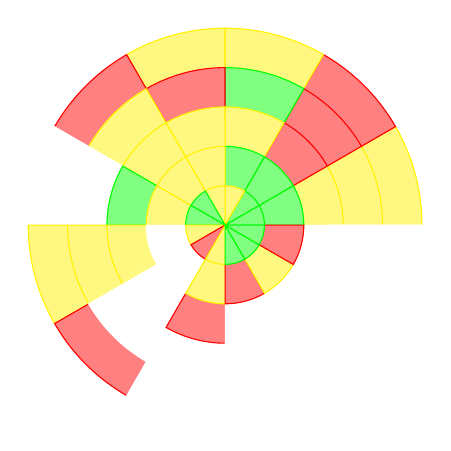
\begin{tikzpicture}[nodes = {font=\sffamily}]
      \foreach \color in {
            yellow,
            red,
            yellow,
            white,
            red,
            yellow,
            white,
            yellow,
            white,
            white,
            red,
            red,
        } {
        \ifx\color\empty\else
            \draw[fill={\color!50},draw={\color}] (0,0) -- (\angle:\radius)
              arc (\angle:\angle+30:\radius) -- cycle;
            \pgfmathparse{\angle+30}
            \xdef\angle{\pgfmathresult}
        \fi
        };
        \xdef\radius{2.5}
        \foreach \color in {
            yellow,
            red,
            yellow,
            yellow,
            red,
            white,
            yellow,
            red,
            white,
            white,
            white,
            white,
        } {
        \ifx\color\empty\else
            \draw[fill={\color!50},draw={\color}] (0,0) -- (\angle:\radius)
              arc (\angle:\angle+30:\radius) -- cycle;
            \pgfmathparse{\angle+30}
            \xdef\angle{\pgfmathresult}
        \fi
        };
        \xdef\radius{2}
        \foreach \color in {
            yellow,
            red,
            green,
            red,
            yellow,
            white,
            yellow,
            white,
            white,
            white,
            white,
            white,
        } {
        \ifx\color\empty\else
            \draw[fill={\color!50},draw={\color}] (0,0) -- (\angle:\radius)
              arc (\angle:\angle+30:\radius) -- cycle;
            \pgfmathparse{\angle+30}
            \xdef\angle{\pgfmathresult}
        \fi
        };
        \xdef\radius{1.5}
        \foreach \color in {
            yellow,
            red,
            yellow,
            yellow,
            yellow,
            green,
            yellow,
            white,
            red,
            white,
            white,
            white,
        } {
        \ifx\color\empty\else
            \draw[fill={\color!50},draw={\color}] (0,0) -- (\angle:\radius)
              arc (\angle:\angle+30:\radius) -- cycle;
            \pgfmathparse{\angle+30}
            \xdef\angle{\pgfmathresult}
        \fi
        };
        \xdef\radius{1}
        \foreach \color in {
            green,
            green,
            green,
            yellow,
            yellow,
            yellow,
            white,
            white,
            yellow,
            red,
            yellow,
            red,
        } {
        \ifx\color\empty\else
            \draw[fill={\color!50},draw={\color}] (0,0) -- (\angle:\radius)
              arc (\angle:\angle+30:\radius) -- cycle;
            \pgfmathparse{\angle+30}
            \xdef\angle{\pgfmathresult}
        \fi
        };
        \xdef\radius{0.5}
        \foreach \color in {
            green,
            green,
            yellow,
            yellow,
            green,
            green,
            yellow,
            red,
            yellow,
            green,
            green,
            green,
        } {
        \ifx\color\empty\else
            \draw[fill={\color!50},draw={\color}] (0,0) -- (\angle:\radius)
              arc (\angle:\angle+30:\radius) -- cycle;
            \pgfmathparse{\angle+30}
            \xdef\angle{\pgfmathresult}
        \fi
        };
    \end{tikzpicture}
\caption{Typical gateway coverage\cite{lorajambalaya}}
\label{fig:coverage}

\begin{tabular}{r@{: }l r@{: }l}
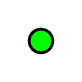
\begin{tikzpicture}\draw[fill=green,line width=1pt]  circle(1ex);\end{tikzpicture} & Good\ Connection & 
\begin{tikzpicture}\draw[fill=yellow,line width=1pt]  circle(1ex);\end{tikzpicture} & Intermediate\ Connection\\
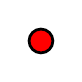
\begin{tikzpicture}\draw[fill=red,line width=1pt]  circle(1ex);\end{tikzpicture} & Bad\ Connection & 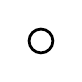
\begin{tikzpicture}\draw[fill=white,line width=1pt]  circle(1ex);\end{tikzpicture} & No\ Connection 
\end{tabular}
\end{figure}




% \begin{tikzpicture}
%     \node[draw] (Application) [abstract, rectangle]{\textbf{Application Layer}};
%     \node[draw] (MAC) [abstract, rectangle, below=0.2cm of Application, text justified]{\textbf{Media Access Control (MAC) Layer}};
%     \node[draw] (Phy) [abstract, rectangle, below=0.2cm of MAC, text justified]{\textbf{Physical (PHY) Layer}};
%     \node[draw] (Rf) [abstract, rectangle, below=0.2cm of Phy, text justified]{\textbf{Radio Frequency (RF) Layer}};
% \end{tikzpicture}

\paragraph{}


Using a multi-hop routing protocol (Fig~\ref{fig:meshtopology}) solution
could mitigate LoRaWAN congestion issues (\cite{8115756}).
Increasing the redundancy and the reliability of the lossy network could be a
solution to the problems previously exposed like varying topology,
environmental changing conditions or end-of-reach devices.
A multi-hop network can adapt to this kind of variation, routing protocols can
keep track and change packets routes for not responding nodes
% TODO {Maybe cite study with the node in water roover}
Also multi-hop is a strong candidate for large areas monitoring application
where few gateways may be available.

Work to create multi-hop routing protocol with LoRa has already been
done in~\cite{8115756} but didn't took into account the energy consumption of
the motes.
Medium Access Control (MAC) protocols such as \emph{TSCH} have
already been developed for the \emph{IEEE 802.15.4} standard to solve the
energy consumption problem.
Work in~\cite{8847137} and~\cite{njomgang_2018} has already been done in
\emph{VUB} to adapt TSCH for LoRa.
This thesis is part of the outcome of the combined efforts of the previous
years by adapting \emph{TSCH} for the \emph{Zoleratia RE-Mote} working with a
\emph{RN2483} LoRa shield.
